% nstab_transition.tex -- round 451, transition anatomy at n_stab.
% TRANSITION_SMOOTH / RES_MISMATCH / PREFIX_Q_PLATEAU.
% Builds with pdflatex.
% Companion machine check: verify_nstab_transition.py.
% Discovery: experiments/tfpt-discovery/nstab_transition_probe.py.
% NO RH CLAIM.  NO anti-RH claim.
\documentclass[11pt]{article}

\usepackage[a4paper,margin=2.7cm]{geometry}
\usepackage{amsmath,amssymb,amsthm}
\usepackage{microtype}
\usepackage{booktabs}
\usepackage{xcolor}
\usepackage{pgfplots}
\pgfplotsset{compat=1.17}
\usepackage[colorlinks=true,linkcolor=blue!50!black,urlcolor=blue!50!black]{hyperref}

\newtheorem{lemma}{Lemma}
\newtheorem{prop}{Proposition}
\newtheorem{definition}{Definition}

\title{\bfseries Transition anatomy at $n_{\mathrm{stab}}$\\[2mm]
\large TRANSITION\_SMOOTH: no universal cliff;\\
the Schur plateau is the stable prefix}
\author{Stefan Hamann}
\date{August 30, 2026}

\begin{document}
\maketitle

\begin{abstract}\noindent
The Prefix Stability Theorem candidate needs a
property that is stable on the early chain and
may be lost later.
This note compares three single-window objects,
profiled in rank $n$ and centred on the r449
cut $n_{\mathrm{stab}}$:
the OP conditioning/Christoffel regime;
fold-atom Nyquist $n_{\mathrm{res}}$;
and the compressed dual-resolvent energy
$q^{\dagger}_n$.
None of the three kinks universally at
$n_{\mathrm{stab}}$ (TRANSITION\_SMOOTH).
Atom Nyquist is $L/2$ and
$n_{\mathrm{stab}}/n_{\mathrm{res}}\in[0.010,0.094]$
(RES\_MISMATCH): the prefix is bandlimited.
What \emph{is} stable on $n\le n_{\mathrm{stab}}$
of every measured window is a constant Schur
value $q^{\dagger}_n\equiv q_*<1$
(PREFIX\_Q\_PLATEAU).
$n_{\mathrm{stab}}$ is a sufficient operational
cut for that plateau, not a unique mechanical
cliff.
No RH claim.  No anti-RH claim.
\end{abstract}

\medskip\noindent
\textbf{Status.}\enspace
No new SATZ.
Propositions~\ref{prop:nres}--\ref{prop:scr}
are a named infra census.
Ausgang
\texttt{TRANSITION\_SMOOTH / RES\_MISMATCH / PREFIX\_Q\_PLATEAU}.
No $L^{*}$ claim.  No $R^{\dagger}$ claim.
No RH claim.  No anti-RH claim.

\section{Objects}\label{sec:obj}

$n_{\mathrm{stab}}$ is the r449 Fenster-Vergleich
(Chebyshev moments of folded $\tilde\mu$, skip
$m_0,m_1$, first neighbour break; the cut is
identical from $\varepsilon=10^{-6}$ to
$10^{-2}$).  It is \emph{not} redefined here.

\begin{definition}[$n_{\mathrm{res}}$, source-pure]\label{def:nres}
Let $\{x_i\}$ be the folded $\mu$-atoms of the
window, $x_i\in[-1,1]$.
Set $\theta_i=\arccos(x_i)$ and
\[
n_{\mathrm{res}}
=\pi\big/\min_i(\theta_{i+1}-\theta_i)
\]
after sorting unique angles.
No fit degree of freedom.
On the cosine grid of the fold this equals
$L/2$.
\end{definition}

\begin{definition}[$q^{\dagger}_n$]\label{def:q}
The r362/r369 pack cut at depth $n$:
$\mu$-chain plus smooth-border augmentation,
$B_w=\mathrm{cumsum}(\rho)[n-2]+5/7$,
$q^{\dagger}=\|\,\cdot\,\|$, $\delta=1-q^{\dagger}$.
$n_{\mathrm{qbreak}}$ is the first $n>n_{\mathrm{ref}}$
with $|q_n-q_{\mathrm{ref}}|>10^{-4}$.
\end{definition}

\section{Conditioning}\label{sec:cond}

\begin{prop}[No Christoffel cliff]\label{prop:cond}
On kz$17$, $136$, $137$, $197$, the Jacobi
couplings stay $\beta_n\approx 1/2$ through
$n_{\mathrm{stab}}$ and
$n\,\lambda_n(0)\in[2.3,6.9]$ (continuous
regime).
A slope-break of $|\beta_n-1/2|$ is not
peaked within $15\%$ of $n_{\mathrm{stab}}$
with ratio $>4$.
The discrete near-singularity of the OP
chain sits near $n_{\mu}\gg n_{\mathrm{stab}}$.
\end{prop}

\section{Resolution}\label{sec:res}

\begin{center}
\small
\begin{tabular}{rrrrrr}
\toprule
$k_z$ & $N$ & $n_{\mathrm{stab}}$ & $n_{\mathrm{res}}$
& $n_{\mathrm{stab}}/n_{\mathrm{res}}$ & $n_{\mathrm{qbreak}}$ \\
\midrule
5 & 72 & 13 & 143 & 0.091 & 24 \\
9 & 184 & 13 & 367 & 0.035 & 46 \\
17 & 96 & 18 & 191 & 0.094 & 19 \\
26 & 364 & 46 & 727 & 0.063 & 60 \\
43 & 839 & 60 & 1677 & 0.036 & 119 \\
69 & 5690 & 119 & 11379 & 0.010 & $>$2$n_{\mathrm{stab}}$ \\
116 & 1433 & 158 & 2865 & 0.055 & 159 \\
136 & 1641 & 175 & 3281 & 0.053 & 176 \\
137 & 8300 & 175 & 16599 & 0.011 & $>$2$n_{\mathrm{stab}}$ \\
170 & 5771 & 194 & 11541 & 0.017 & $>$2$n_{\mathrm{stab}}$ \\
197 & 4071 & 406 & 8141 & 0.050 & 407 \\
230 & 2012 & 194 & 4023 & 0.048 & 195 \\
500$^{\mathrm{f}}$ & 17847 & 1525 & 35693 & 0.043 & 1526 \\
\bottomrule
\end{tabular}
\end{center}

$^{\mathrm{f}}$float Gram; residual $1.5\cdot10^{-15}$
at $n_{\mathrm{stab}}$.

\begin{prop}[RES\_MISMATCH]\label{prop:nres}
On every measured window,
$n_{\mathrm{stab}}/n_{\mathrm{res}}\in[0.010,0.094]$.
The prefix does not resolve individual fold
atoms.
Hypothesis $n_{\mathrm{stab}}\approx n_{\mathrm{res}}$
is false.
The weaker bandlimited statement holds:
the extraction prefix sits well below Nyquist.
\end{prop}

\begin{center}
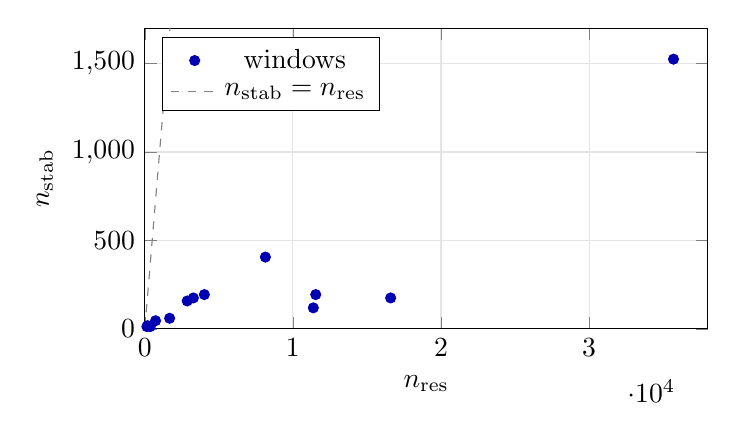
\begin{tikzpicture}
\begin{axis}[
  width=0.72\textwidth, height=5.4cm,
  xlabel={$n_{\mathrm{res}}$},
  ylabel={$n_{\mathrm{stab}}$},
  xmin=0, xmax=38000, ymin=0, ymax=1700,
  legend pos=north west,
  grid=major, grid style={gray!20},
]
\addplot[only marks, mark=*, mark size=1.8pt, blue!70!black]
  coordinates {
    (143,13) (367,13) (191,18) (727,46) (1677,60)
    (11379,119) (2865,158) (3281,175) (16599,175)
    (11541,194) (8141,406) (4023,194) (35693,1525)
  };
\addlegendentry{windows}
\addplot[domain=0:38000, dashed, gray] {x};
\addlegendentry{$n_{\mathrm{stab}}=n_{\mathrm{res}}$}
\end{axis}
\end{tikzpicture}
\end{center}

\section{Schur energy}\label{sec:schur}

\begin{prop}[PREFIX\_Q\_PLATEAU]\label{prop:q}
On every measured window, including kz$137/170/500$,
$q^{\dagger}_n$ is constant for $n\le n_{\mathrm{stab}}$
(plateau std $<10^{-4}$, Gram residual
$\le 10^{-14}$, $q_*<1$).
The uniform bound
$q^{\dagger}_n\le q_*<1$ therefore holds on the
r449 prefix.
The \emph{exit} of the plateau is not a
universal cliff at $n_{\mathrm{stab}}$:
CLIFF at $n_{\mathrm{stab}}{+}1$ on
$\{17,116,136,197,230,500\}$;
DELAYED on $\{5,9,26,43\}$;
CONTINUES past $2\,n_{\mathrm{stab}}$ on
$\{69,137,170\}$.
\end{prop}

\begin{center}
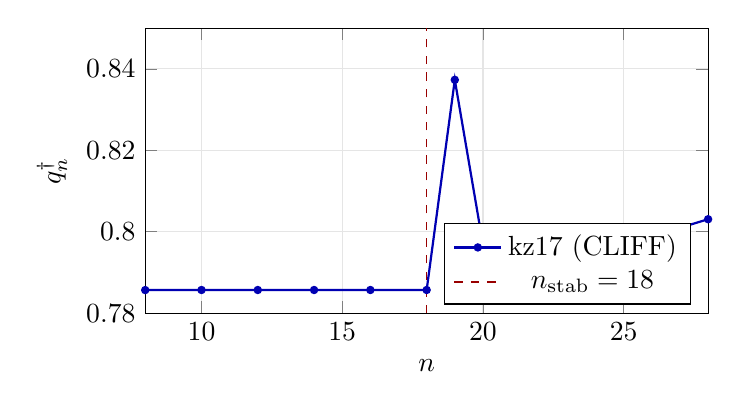
\begin{tikzpicture}
\begin{axis}[
  width=0.72\textwidth, height=5.2cm,
  xlabel={$n$},
  ylabel={$q^{\dagger}_n$},
  xmin=8, xmax=28, ymin=0.78, ymax=0.85,
  legend pos=south east,
  grid=major, grid style={gray!20},
]
\addplot[thick, blue!70!black, mark=*, mark size=1.1pt]
  coordinates {
    (8,0.78566) (10,0.78568) (12,0.78568) (14,0.78568)
    (16,0.78568) (18,0.78568) (19,0.83732) (20,0.79689)
    (22,0.79911) (24,0.80082) (26,0.79886) (28,0.80307)
  };
\addlegendentry{kz17 (CLIFF)}
\addplot[dashed, red!60!black]
  coordinates {(18,0.78) (18,0.85)};
\addlegendentry{$n_{\mathrm{stab}}=18$}
\end{axis}
\end{tikzpicture}
\end{center}

kz$136$ (live, $N=1641$): $q_{175}=0.87092$,
$q_{176}=0.87551$ (CLIFF).
kz$137$ (dead tail, $N=8300$, same
$n_{\mathrm{stab}}=175$): $q$ stays $0.90011$
through $n=369$ (CONTINUES).
Same cut, different exit --- the cliff is not
the definition of $n_{\mathrm{stab}}$.

\section{Scramble}\label{sec:scr}

\begin{prop}[Construction-specific plateau]\label{prop:scr}
Theta-jitter of kz$17$ (seed $451$):
$n_{\mathrm{stab}}\to 2$,
$n_{\mathrm{res}}$ blows up to $9\cdot10^5$,
$q^{\dagger}_n$ wanders (std $0.09$, max $>1$).
The live plateau is fold-arithmetic, not a
generic OP artefact of $138$ atoms.
The live $n_{\mathrm{res}}$-mismatch survives
(scramble still has $n_{\mathrm{stab}}\ll n_{\mathrm{res}}$):
Nyquist is support geometry; $n_{\mathrm{stab}}$
and the plateau are the window comparison.
\end{prop}

\section{Consequence for the theorem candidate}\label{sec:thm}

$n_{\mathrm{stab}}$ is a \emph{measurement cut}
(neighbour-moment disagreement), not a unique
mechanical cliff of conditioning or of atom
resolution.
It is nevertheless a \emph{sufficient} depth:
on $n\le n_{\mathrm{stab}}$ the compressed
$R^{\dagger}$ is positivity-compatible
($q^{\dagger}_n\equiv q_*<1$) and bandlimited
($n\ll n_{\mathrm{res}}$).
The Prefix Stability Theorem can name that
plateau; it cannot claim that instability
begins exactly at the cut.

\section*{Claim boundary}

Nothing here is evidence for or against the
Riemann hypothesis, in either direction.
The identities are a finite moment/chain/pack
census.

\begin{thebibliography}{9}
\bibitem{r449} Flip versus stabilization; $n_{\mathrm{stab}}$.
\bibitem{r445} Slice floor; $q^{\dagger}$ pack.
\bibitem{r450} Prefix mincut; $n_{\mathrm{stab}}$-compression.
\end{thebibliography}

\end{document}
